\documentclass[11pt, a4paper]{article}
\usepackage[utf8]{inputenc}
\usepackage{calc}
\usepackage[T1]{fontenc}
\usepackage{geometry}
\usepackage{graphicx}
\usepackage{hyperref}
\usepackage{amsmath}
\usepackage{booktabs}
\usepackage{tabularx}
\usepackage{multirow}
\usepackage[sort&compress]{natbib}
\usepackage[french]{babel}
\usepackage{enumitem}
\usepackage{float}


\geometry{margin=2.5cm}
\setlength{\parskip}{0.5em}

\begin{document}

\begin{titlepage}
    \centering
    \begin{figure}[h]
        \centering
        
\includegraphics[width=0.5\textwidth]{./assets/logo_polymtl.png}
        \label{fig:logo_polymtl}
    \end{figure}

    {\scshape\LARGE Polytechnique Montréal \par}
    \vspace{1cm}
    {\scshape\Large INF8245AE – Machine Learning \par}
    \vspace{4cm}
    {\huge\bfseries Assignment 1 – Linear Regression\par}
    \vspace{2cm}
    {\Large\itshape Mattéo Colavita - 2142009\par}
    \vfill
    \vspace{0.8cm}
    {\large 2025-09-26\par}
\end{titlepage}

\section{Question 1: Linear and Weighted Ridge Regression}

\begin{figure}[H]
\centering
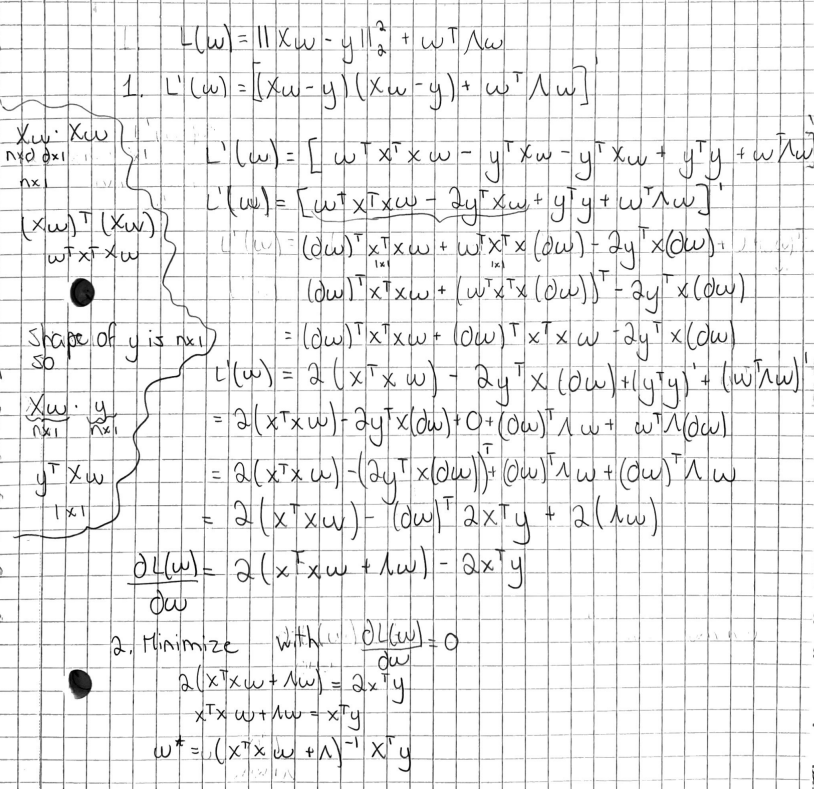
\includegraphics[width=0.6\textwidth]{./assets/derivative.png}
\caption{Derivative of the loss function for ridge regression with respect to the weights.}
\label{fig:derivative}
\end{figure}

\begin{figure}[H]
\centering
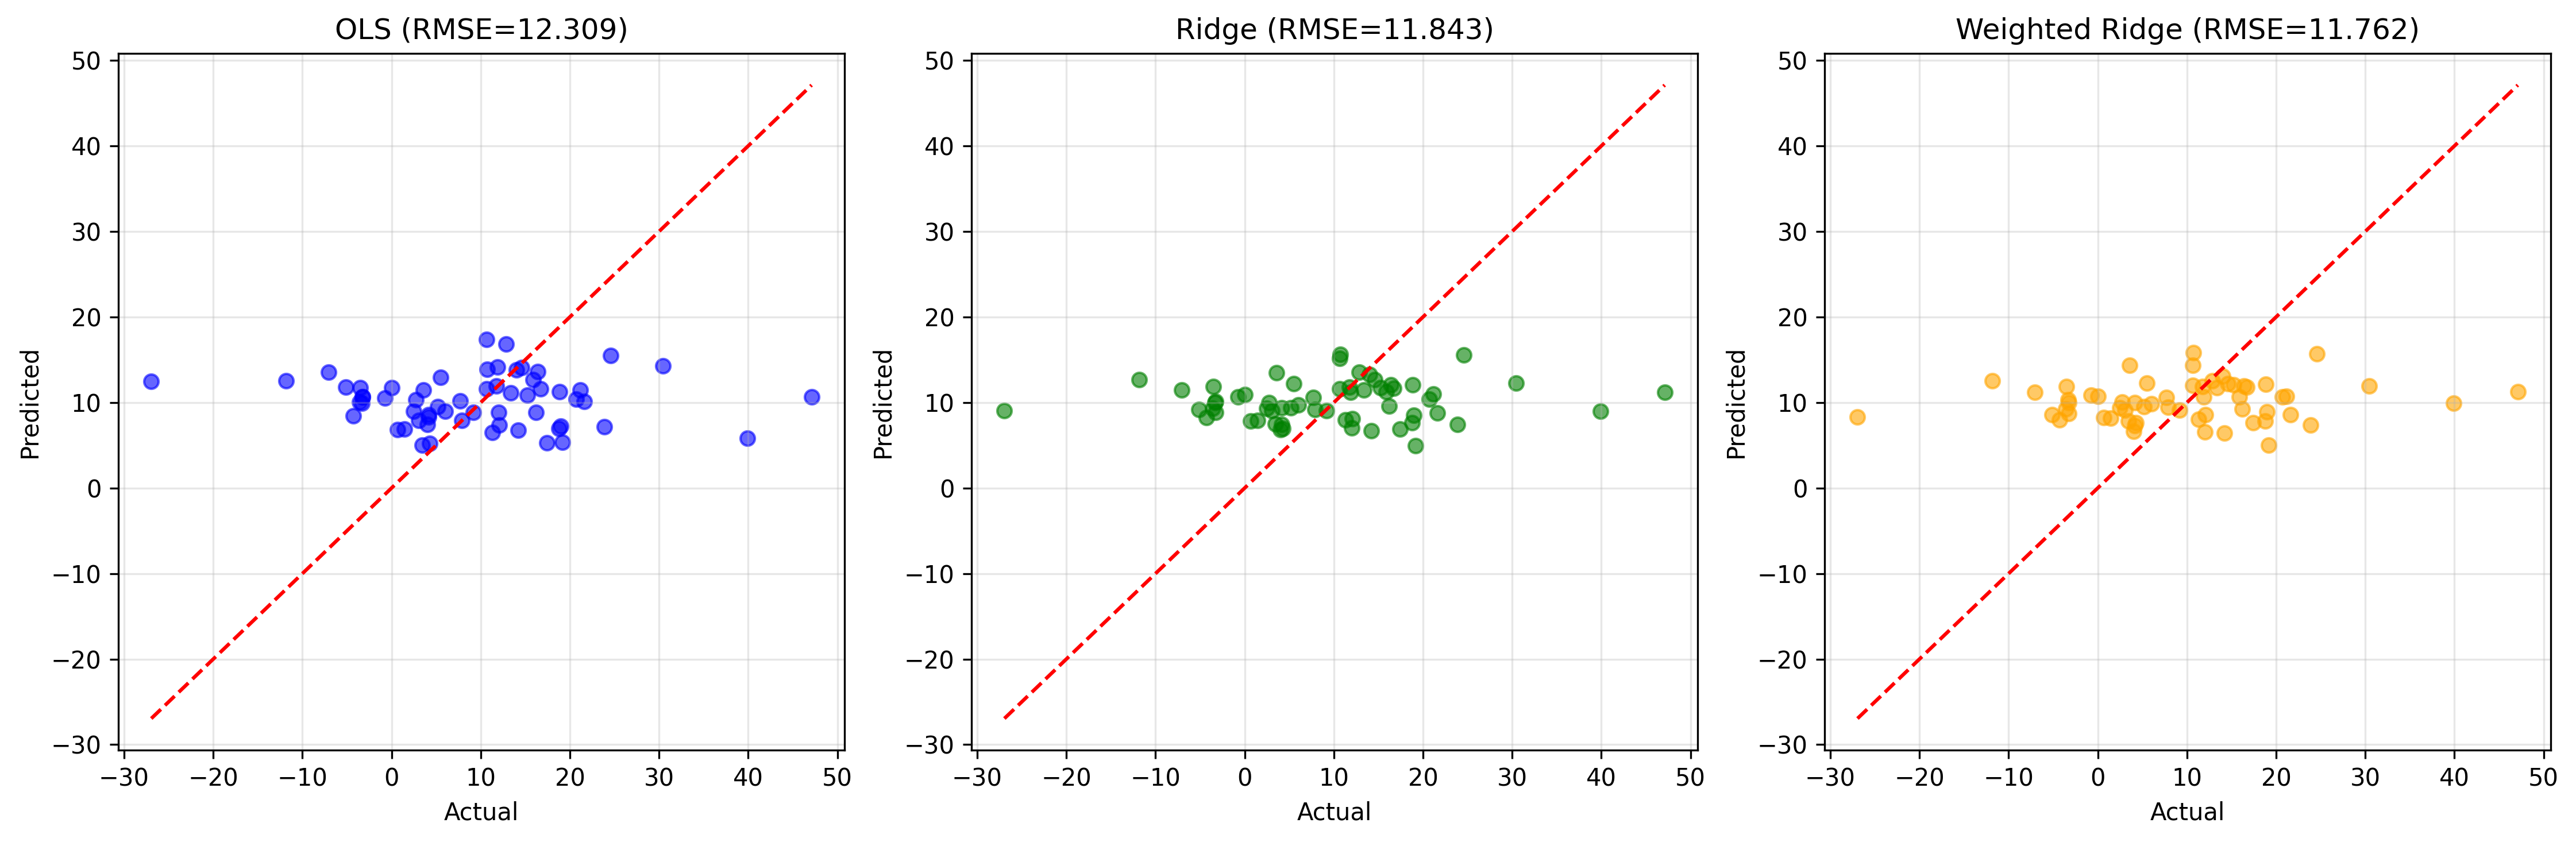
\includegraphics[width=1\textwidth]{./assets/regression_comparison.png}
\caption{Comparison of predictions from linear, ridge and weighted ridge regression on the test set.}
\label{fig:linear_vs_weighted_ridge}
\end{figure}

\section{Question 2: Cross-Validation}

\begin{table}[H]
\centering
\begin{tabular}{|l|c|c|c|c|c|c|}
\hline
\textbf{Metric} & \textbf{Best $\lambda$} & \textbf{$\lambda$=0.01} & \textbf{$\lambda$=0.1} & \textbf{$\lambda$=1} & \textbf{$\lambda$=10} & \textbf{$\lambda$=100} \\
\hline
MAE & 10 & 7.381 & 7.316 & 7.140 & 7.110 & 7.817 \\
\hline
MaxError & 100 & 27.758 & 27.681 & 27.559 & 27.476 & 27.095 \\
\hline
RMSE & 10 & 9.855 & 9.772 & 9.577 & 9.532 & 10.101 \\
\hline
\end{tabular}
\caption{Mean MAE, MaxError, and RMSE scores obtained via 5-fold cross-validation for different values of $\lambda$ in ridge regression.}
\label{tab:cross_validation_results}
\end{table}

\section{Question 3: Gradient Descent for Ridge Regression}

\begin{figure}[H]
    \centering
    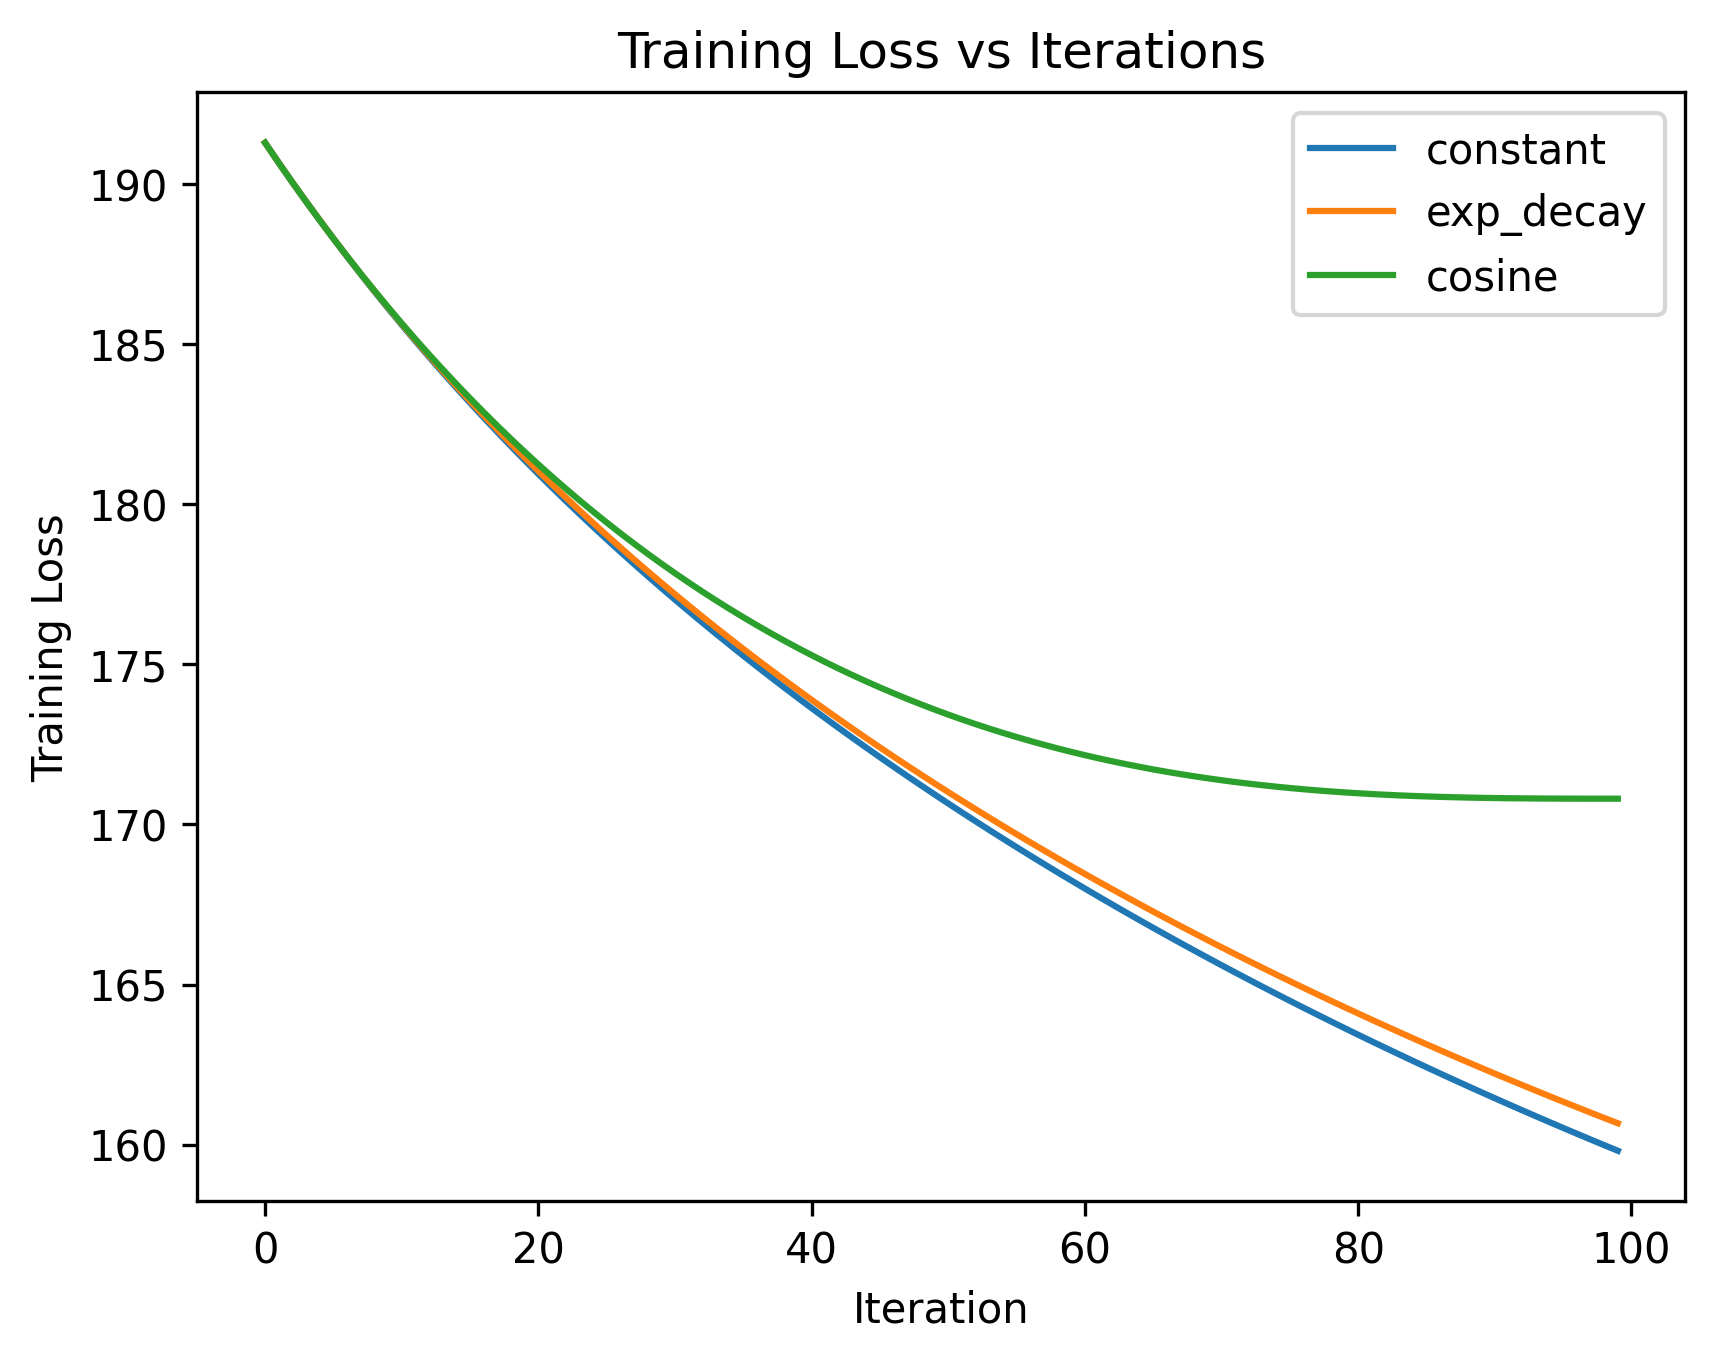
\includegraphics[width=0.8\textwidth]{./assets/training_loss_comparison.png}
    \caption{Training loss vs iterations for different learning rate schedules in gradient descent for ridge regression.}
    \label{fig:training_loss_comparison}
\end{figure}

\begin{table}[h!]
\centering
\begin{tabular}{|l|c|}
\hline
\textbf{Learning Rate Schedule} & \textbf{RMSE} \\
\hline
Constant & 13.8910 \\
\hline
Exponential Decay & 13.9283 \\
\hline
Cosine Annealing & 14.3473 \\
\hline
\end{tabular}
\caption{RMSE results for different learning rate schedules in gradient descent for ridge regression.}
\label{tab:learning_rate_schedules}
\end{table}

Among the tested learning rate schedules, both constant and exponential decay schedules show a fast decrease in training
loss and achieved low RMSE values of 13.89 and 13.93, suggesting great generalization. In contrast, cosine annealing plateaued early,
indicating premature convergence at a suboptimal point. The rapid decay of the learning rate within the given amount of iterations
may have caused smaller step sizes before reaching the minimum, preventing stable convergence despite ridge regression's convex loss function.

\end{document}

